%!TEX root = paper/paper.tex
\section{Experiments}

% Details of our experiments follow, with a concluding discussion section.
% Due to space constraints, we are not able to provide as many figures as we would like here; however, the Supplementary Materials provides a full accounting.

\begin{table}
\caption{
    Mean APs on three datasets for the considered single-channel features and their second-stage combination.
    As some features were clearly worse than others on the AVA Style dataset, only the better features were evaluated on larger datasets.
}
\label{tab:mean_aps}
\centering
\vspace{1em}
\footnotesize{
\begin{tabular}{lrrrrrrrrr}
\toprule
{}                & Fusion x Content & DeCAF$_6$ & MC-bit & L*a*b* Hist & GIST  & Saliency & random \\
\midrule
AVA Style         & \textbf{0.581}   & 0.579     & 0.539  & 0.288       & 0.220 & 0.152    & 0.132 \\
Flickr            & \textbf{0.368}   & 0.336     & 0.328  & -           & -     & -        & 0.052 \\
Wikipaintings     & \textbf{0.473}   & 0.356     & 0.441  & -           & -     & -        & 0.043 \\
\bottomrule
\end{tabular}
}
\end{table}


\subsection{Flickr Style}
We learn and predict style labels on the 80,000 images labeled with 20 different visual styles of our new Flickr Style dataset, using 20\% of the data for testing, and another 20\% for parameter-tuning validation.

There are several performance metrics we consider.
Average Precision evaluation (as reported in \autoref{tab:mean_aps} and in detailed tables in the Supplementary Materials) is computed on a random class-balanced subset of the test data (each class has equal prevalence).
We compute confusion matrices on the same data.
Per-class accuracies are computed on subsets of the data balanced by the binary label, such that chance performance is 50\%.
We follow these decisions in all following experiments.

The best single-channel feature is DeCAF$_6$ with 0.336 mean AP; feature fusion obtains 0.368 mean AP.
Per-class APs range from 0.17 [Depth of Field] to  0.62 [Macro].
Per-class accuracies range from 68\% [Romantic, Depth of Field] to 85\% [Sunny, Noir, Macro].
The average per-class accuracy is 78\%.
We show the most confident style classifications on the test set of Flickr Style in \autoref{fig:flickr_on_flickr}.

Upon inspection of the confusion matrices, we saw points of understandable confusion: Depth of Field vs.~Macro, Romantic vs.~Pastel, Vintage vs.~Melancholy.
There are also surprising sources of mistakes: Macro vs.~Bright/Energetic, for example.
To explain this particular confusion, we observed that lots of Macro photos contain bright flowers, insects, or birds, often against vibrant greenery.
Here, at least, the content of the image dominates its style label.

To explore further content-style correlations, we plot the outputs of PASCAL object class classifiers (one of our features) on the Flickr dataset in~\autoref{fig:content_correlation}.
We can observe that some styles have strong correlations to content (e.g., ``Hazy'' occurs with ``vehicle'', ``HDR'' doesn't occur with ``cat'').

We hypothesize that style is content-dependent: a Romantic portrait may have different low-level properties than a Romantic sunset. We form a new feature as an outer product of our content classifier features with the second-stage late fusion features (``Fusion $\times$ Content'' in all results figures).  These features gave the best results, thus supporting the hypothesis.

\begin{figure}[h]
\centering
    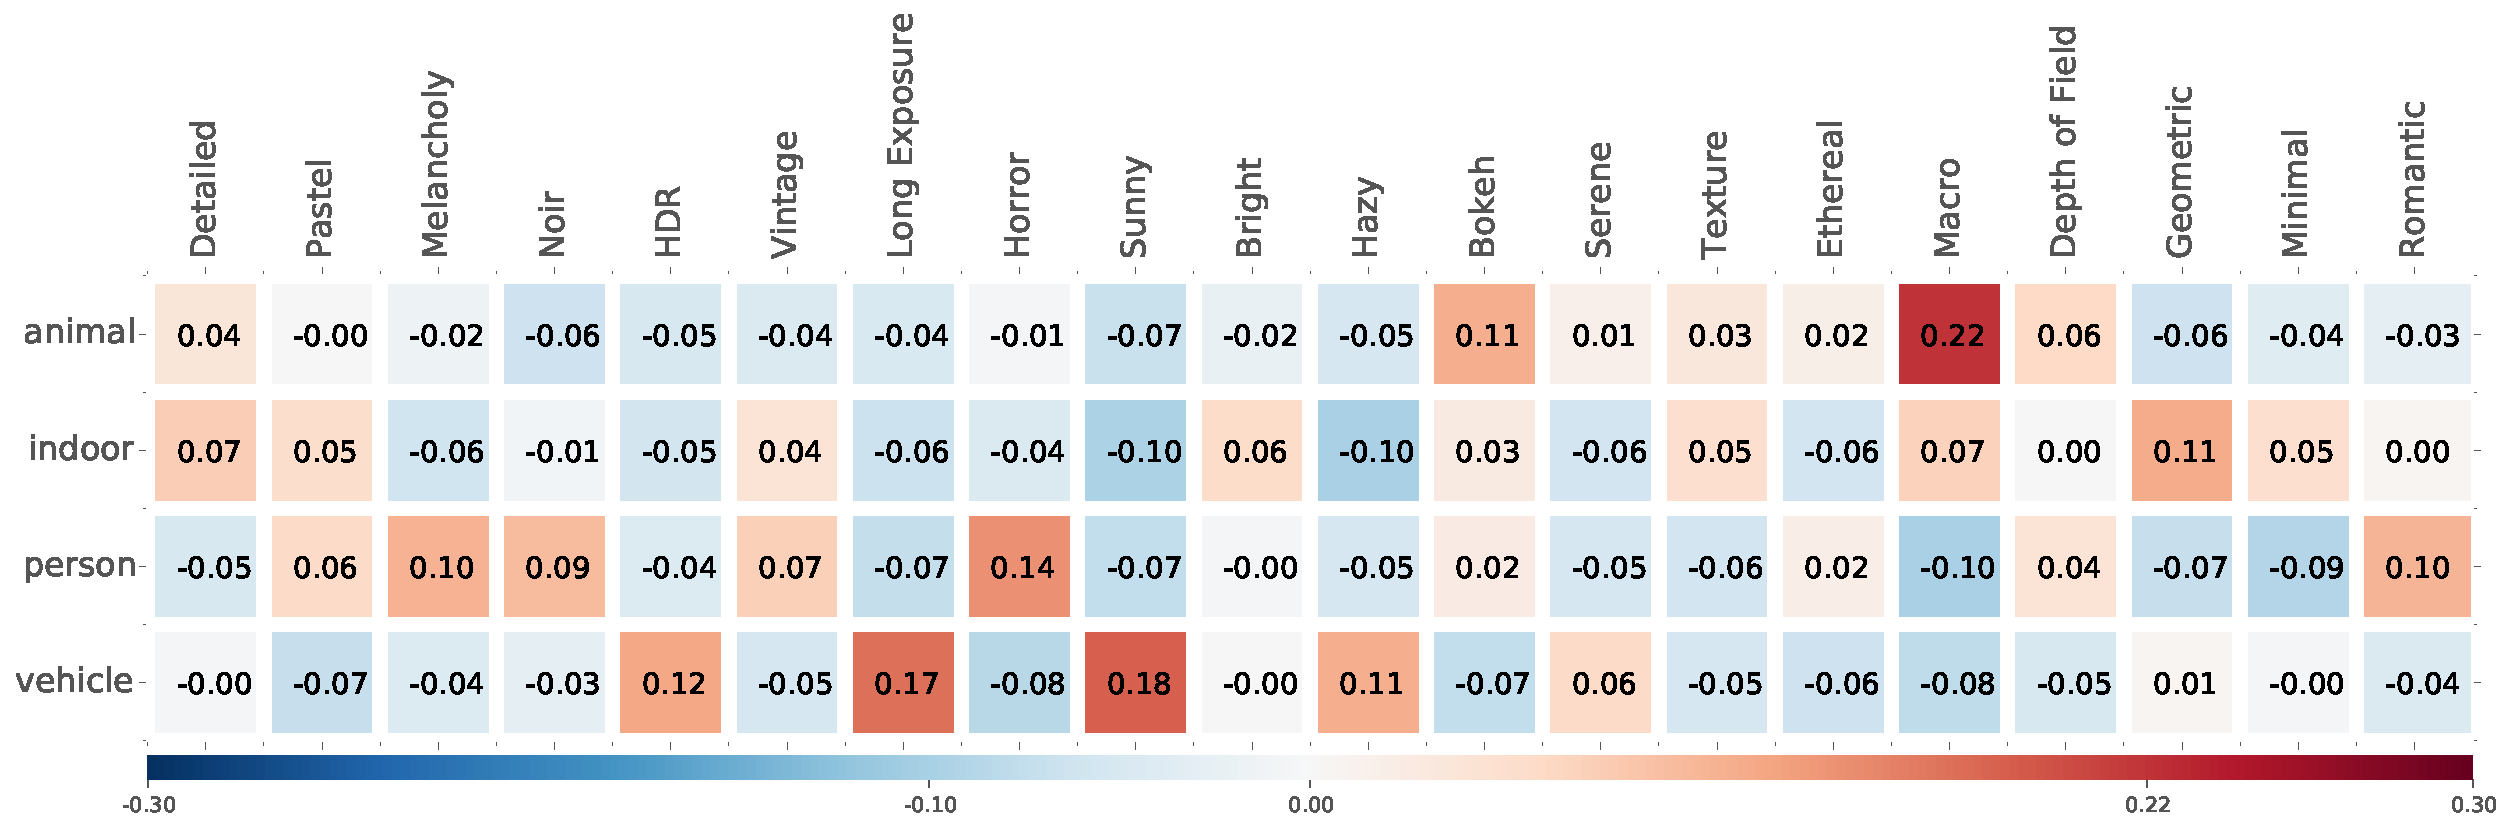
\includegraphics[width=\linewidth]{../../figures/content_correlation2/pascal_on_flickr.pdf}
    \caption{
        Correlation of PASCAL content classifier predictions (rows) against ground truth Flickr Style labels (columns).
        We see, for instance, that the Macro style is highly correlated with presence of animals, and that Long Exposure and Sunny style photographs often feature vehicles.
    }\label{fig:content_correlation}
\end{figure}

\vspace{-.5em}
\paragraph{Mechanical Turk Evaluation.}\label{sec:mech_turk_evaluation}
In order to provide a human baseline for evaluation, we performed a Mechanical Turk study.
For each style, Turkers were shown positive and negative examples for each Flickr Group, and then they evaluated whether each image in the test set was part of the given style.
We treat the Flickr group memberships as ground truth as before, and then evaluate Turkers' ability to accurately determine group membership.
Measures were taken to remove spam workers; see the Supplemental Material details on the experimental setup.
For efficiency, one quarter of the test set was used, and two redundant styles (Bokeh and Detailed) were removed.
Each test image was evaluated by 3 Turkers, and the majority vote taken as the human result for this image.

In total, Turkers achieved 75\% mean accuracy (ranging from 61\% [Romantic] to 92\% [Macro]) across styles, in comparison to 78\% mean accuracy (ranging from 68\% [Depth of Field] to 87\% [Macro]) of our best method.
Our algorithm did significantly worse than Turkers on Macro and Horror, and significantly better on Vintage, Romantic, Pastel, Detailed, HDR, and Long Exposure styles.

Some of this variance may be due to subtle difference from the Turk tasks that we provided, as compared to the definitions of the Flickr groups, but may also due to the Flickr groups' incorporating images that do not quite fit the common definition of the given style.
For example, there may be a mismatch between different notions of ``romantic'' and ``vintage,'' and how inclusively these terms are defined.

We additionally used the Turker opinion as ground truth for our method's predictions.
In switching from the default Flickr to the MTurk ground truth, our method's accuracy hardly changed from 78\% to 77\%.
However, we saw that the accuracy of our Vintage, Detailed, Long Exposure, Minimal, HDR, and Sunny style classifiers significantly decreased, indicating machine-human disagreement on those styles.
Detailed tables are provided in Supplemental Results.

\subsection{Wikipaintings}
With the same setup and features as in the Flickr experiments, we evaluate 85,000 images labeled with 25 different art styles.
The results are given in \autoref{tab:mean_aps} and in Supplementary Materials.
The best single-channel feature is MC-bit with 0.441 mean AP; feature fusion obtains 0.473 mean AP.
Per-class accuracies range from 72\% [Symbolism, Expressionism, Art Nouveau] to 94\% [Ukiyo-e, Minimalism, Color Field Painting].

\subsection{AVA Style}
AVA \cite{Murray-CVPR-2012} is a dataset of 250K images from \texttt{dpchallenge.net}.
We evaluate classification of aesthetic rating and of 14 different photographic style labels on the 14,000 images of the AVA dataset that have such labels.
For the style labels, the publishers of the dataset provide a train/test split, where training images have only one label, but test images may have more than one label \cite{Murray-CVPR-2012}.
For style classification, the best single feature is the DeCAF$_6$ convolution network feature, obtaining 0.579 mean AP.
Feature fusion improves the result to 0.581 mean AP; both results beat the previous state-of-the-art of 0.538 mean AP \cite{Murray-CVPR-2012}.
% \footnote{Our results beat 0.54 mAP using both the AVA-provided class-imbalanced test split, and the class-balanced subsample that we consider to be more correct evaluation, and for which we provide numbers.}

In all metrics, the DeCAF and MC-bit features significantly outperformed more low-level features on this dataset.
Accordingly, we do not evaluate the low-level features on the larger Flickr and Wikipaintings datasets.
